% !TEX root = smc_bandits.tex

We assess in Figure~\ref{fig:dynamic_bandits_logistic_c_M} the impact of Monte Carlo sample size $M$ in the performance of the proposed SMC-based Bayesian MAB policies
in Scenario C defined by Equation~\eqref{eq:linear_mixing_dynamics_c},
for a realization of expected rewards as depicted in Figure~\ref{fig:linear_mixing_dynamics_c_logistic}.

% Scenario C
\begin{figure}[!h]
	\centering
	\begin{subfigure}[b]{0.45\textwidth}
		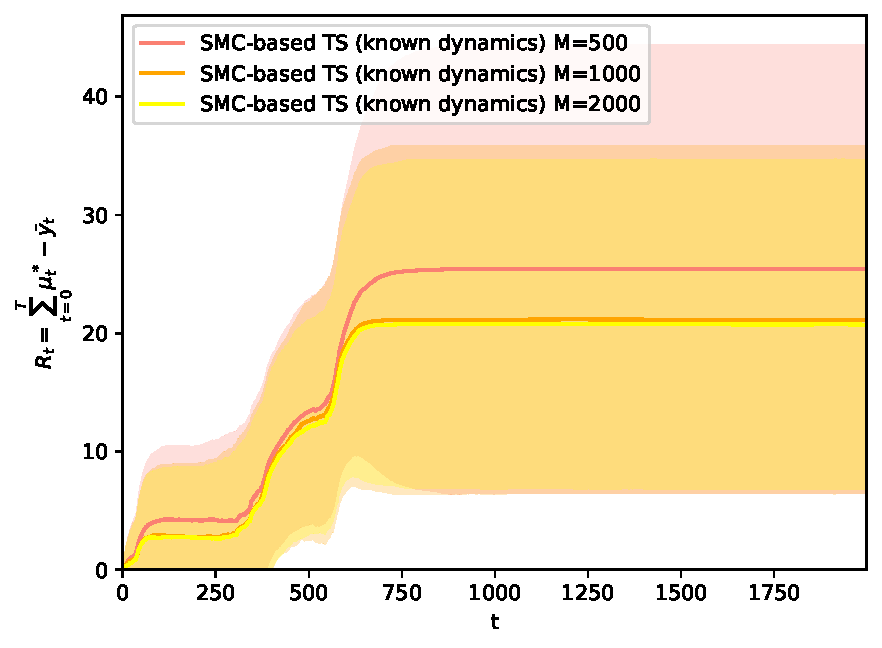
\includegraphics[width=\textwidth]{./fods_figs/dynamic/logistic/c_selectedM_cumulative_regret_dknown_ts}
		\caption{Cumulative regret for SMC-based TS in scenario C: known dynamic parameters.}
		\label{fig:dynamic_bandits_logistic_c_ts_dknown_M}
	\end{subfigure}\qquad
	\begin{subfigure}[b]{0.45\textwidth}
		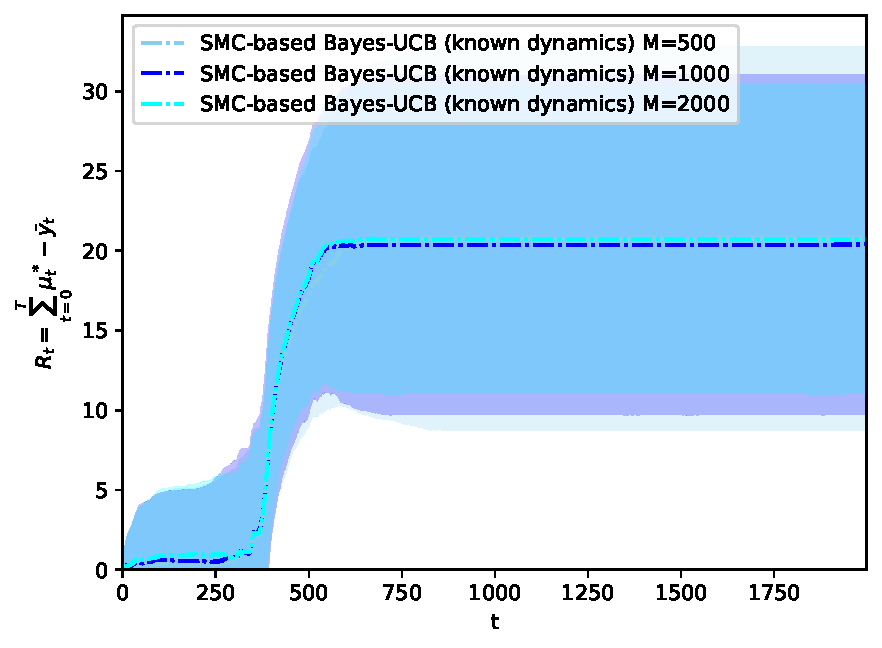
\includegraphics[width=\textwidth]{./fods_figs/dynamic/logistic/c_selectedM_cumulative_regret_dknown_bucb}
		\caption{Cumulative regret for SMC-based Bayes-UCB in scenario C: known dynamic parameters.}
		\label{fig:dynamic_bandits_logistic_c_bucb_dknown_M}
	\end{subfigure}
	
	\begin{subfigure}[b]{0.45\textwidth}
		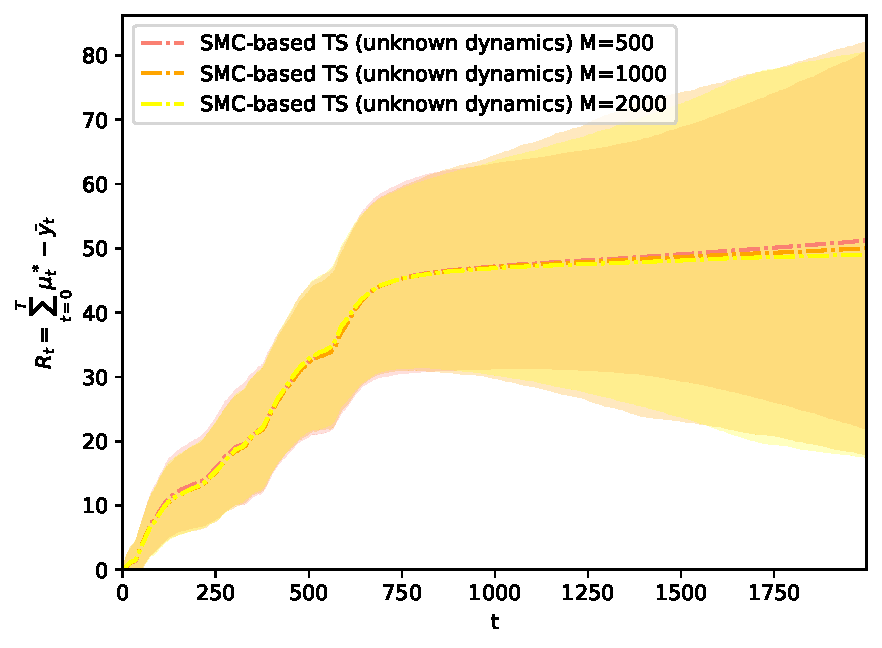
\includegraphics[width=\textwidth]{./fods_figs/dynamic/logistic/c_selectedM_cumulative_regret_dunknown_ts}
		\caption{Cumulative regret for SMC-based TS in scenario C: unknown dynamic parameters $L_a,\Sigma_a,\sigma_a^2, \forall a$.}
		\label{fig:dynamic_bandits_logistic_c_ts_dunknown_M}
	\end{subfigure}\qquad
	\begin{subfigure}[b]{0.45\textwidth}
		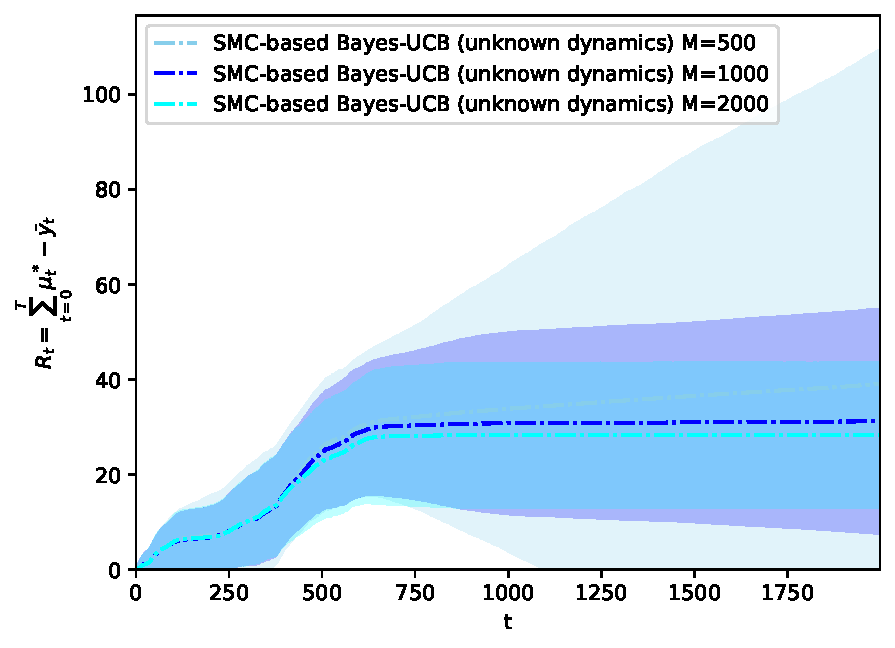
\includegraphics[width=\textwidth]{./fods_figs/dynamic/logistic/c_selectedM_cumulative_regret_dunknown_bucb}
		\caption{Cumulative regret for SMC-based Bayes-UCB in scenario C: unknown dynamic parameters $L_a,\Sigma_a,\sigma_a^2, \forall a$.}
		\label{fig:dynamic_bandits_logistic_c_bucb_dunknown_M}
	\end{subfigure}
	
	\caption{
		Mean regret (standard deviation shown as the shaded region) in contextual, logistic bandit Scenario C
		described in Equation~\eqref{eq:linear_mixing_dynamics_c}.
		SMC-based policies' averaged cumulative regret is robust to different Monte Carlo sample sizes $M$,
		which impacts mostly the performance variability for $M=500$. 
	}
	\label{fig:dynamic_bandits_logistic_c_M}
\end{figure}

\clearpage
We assess in Figure~\ref{fig:dynamic_bandits_logistic_d_M} the impact of Monte Carlo sample size $M$ in the performance of the proposed SMC-based Bayesian MAB policies
in Scenario D defined by Equation~\eqref{eq:linear_mixing_dynamics_c},
for a realization of expected rewards as depicted in Figure~\ref{fig:linear_mixing_dynamics_d_logistic}.

% Scenario D
\begin{figure}[!h]
	\centering
	\begin{subfigure}[b]{0.45\textwidth}
		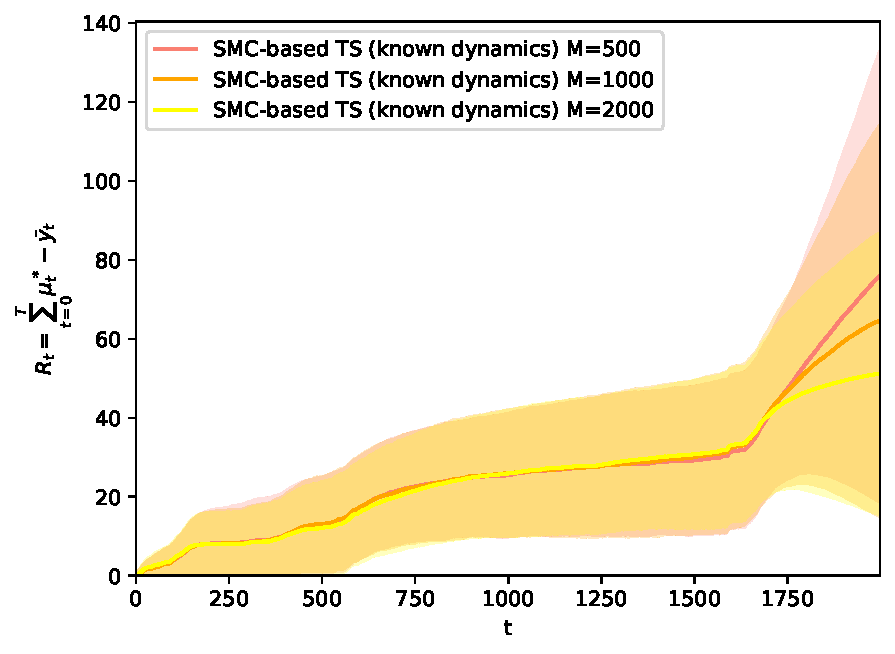
\includegraphics[width=\textwidth]{./fods_figs/dynamic/logistic/d_selectedM_cumulative_regret_dknown_ts}
		\caption{Cumulative regret for SMC-based TS in scenario D: known dynamic parameters.}
		\label{fig:dynamic_bandits_logistic_d_ts_dknown_M}
	\end{subfigure}\qquad
	\begin{subfigure}[b]{0.45\textwidth}
		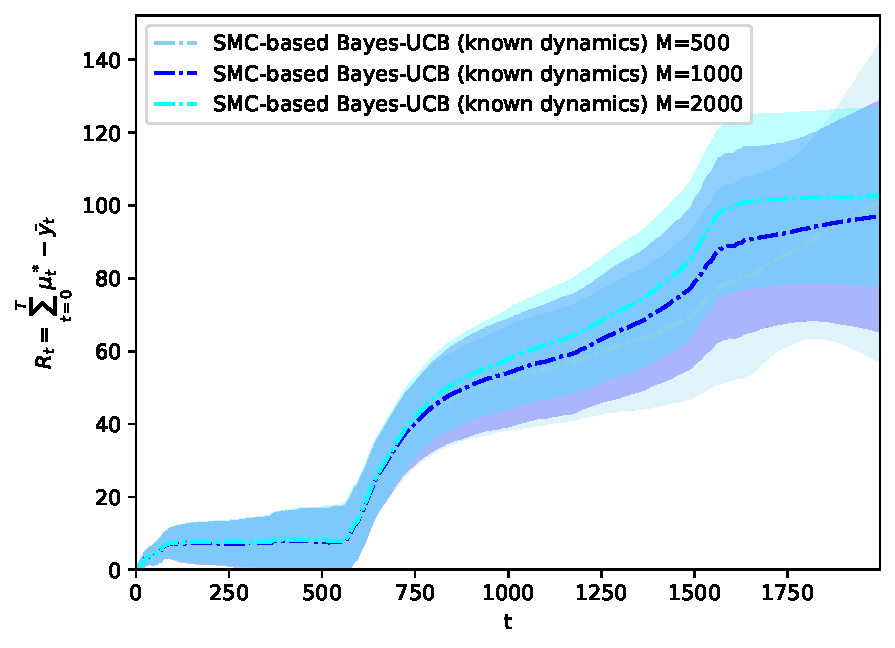
\includegraphics[width=\textwidth]{./fods_figs/dynamic/logistic/d_selectedM_cumulative_regret_dknown_bucb}
		\caption{Dumulative regret for SMC-based Bayes-UCB in scenario D: known dynamic parameters.}
		\label{fig:dynamic_bandits_logistic_d_bucb_dknown_M}
	\end{subfigure}
	
	\begin{subfigure}[b]{0.45\textwidth}
		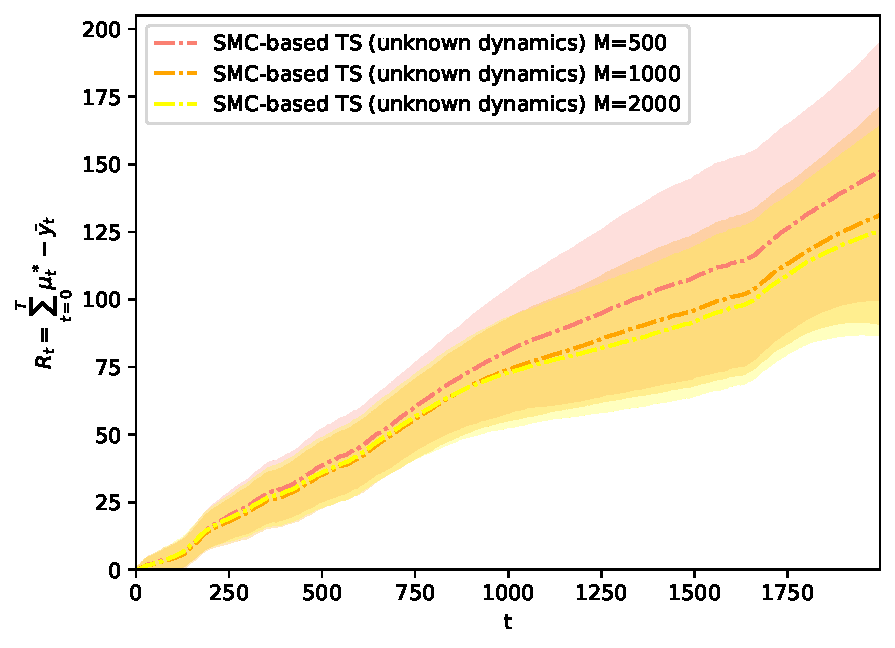
\includegraphics[width=\textwidth]{./fods_figs/dynamic/logistic/d_selectedM_cumulative_regret_dunknown_ts}
		\caption{Cumulative regret for SMC-based TS in scenario D: unknown dynamic parameters $L_a,\Sigma_a,\sigma_a^2, \forall a$.}
		\label{fig:dynamic_bandits_logistic_d_ts_dunknown_M}
	\end{subfigure}\qquad
	\begin{subfigure}[b]{0.45\textwidth}
		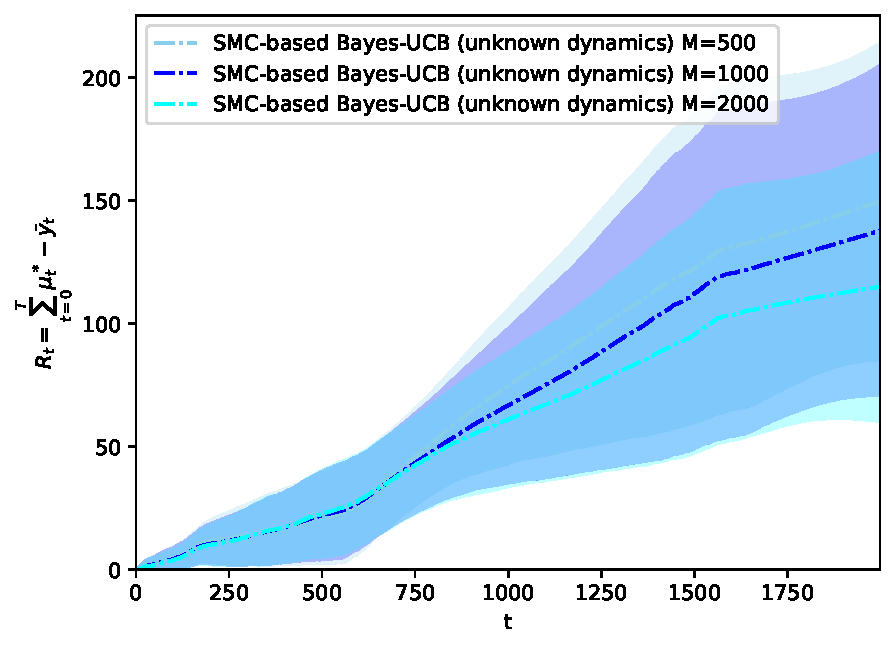
\includegraphics[width=\textwidth]{./fods_figs/dynamic/logistic/d_selectedM_cumulative_regret_dunknown_bucb}
		\caption{Cumulative regret for SMC-based Bayes-UCB in scenario D: unknown dynamic parameters $L_a,\Sigma_a,\sigma_a^2, \forall a$.}
		\label{fig:dynamic_bandits_logistic_d_bucb_dunknown_M}
	\end{subfigure}
	
	\caption{
		Mean regret (standard deviation shown as the shaded region) in contextual, logistic bandit Scenario D
		described in Equation~\eqref{eq:linear_mixing_dynamics_d}.
		SMC-based policies' averaged cumulative regret is robust to different Monte Carlo sample sizes $M$,
		which impacts mostly the performance variability for $M=500$ ---specially so when optimal arm swaps occur later in time.
	}
	\label{fig:dynamic_bandits_logistic_d_M}
\end{figure}
